\documentclass[10pt]{article}

\usepackage{amssymb, amsfonts, amsmath, amsthm}
\usepackage{mathrsfs}
\usepackage{hyperref}
\usepackage{graphicx}
\usepackage{caption}
\usepackage{subcaption}
\usepackage{wrapfig}
\usepackage[margin=1.00 in]{geometry}
\usepackage{enumerate}
\usepackage{harpoon}
\usepackage{nicefrac}
\usepackage{tikz, pgfplots}
\usepackage{xypic}
\usepackage{tikz-cd}
\usepackage{booktabs}

\usepackage{fancyhdr}
\pagestyle{fancy}
\fancyhead{} % clear all header fields
\renewcommand{\headrulewidth}{0pt} % no line in header area
\fancyfoot{} % clear all footer fields
\fancyfoot[LE,RO]{\footnotesize \thepage}           % page number in "outer" position of footer line

\pgfplotsset{compat=newest}

%\setlength\parindent{0pt}%removes indents from entire file

\newtheorem*{sol}{Solution}

\newcommand{\N}{\mathbb{N}}
\newcommand{\Z}{\mathbb{Z}}
\newcommand{\R}{\mathbb{R}}
\newcommand{\C}{\mathbb{C}}
\renewcommand{\P}{\mathbb{P}}

\newcommand{\Unif}{\operatorname{Uniform}}
\newcommand{\Bern}{\operatorname{Bernoulli}}
\newcommand{\Binom}{\operatorname{Binomial}}
\newcommand{\Poiss}{\operatorname{Poisson}}
\newcommand{\se}{\operatorname{se}}
\newcommand{\Exp}{\operatorname{Exp}}

\begin{document}

\noindent \large{Solutions to selected exercises from Chapter 2 of
\emph{Wasserman --- All of Statistics}}

\begin{enumerate}
\item[(2)]
The CDF is
\[
F(x) =
    \begin{cases}
      0 & x < 2 \\
      1/10 & 2\leq x\leq 3 \\
      2/10 & 3\leq x \leq 5 \\
      1 & x\geq 5
   \end{cases}
\]
Thus $\P(2<X\leq 4.8) = F(4.8)-F(2)=2/10-1/10=1/10$ and
$\P(2\leq X\leq 4.8)=\P(X=2)+1/10=2/10$. A plot is shown below.

\begin{figure}[h]
\centering
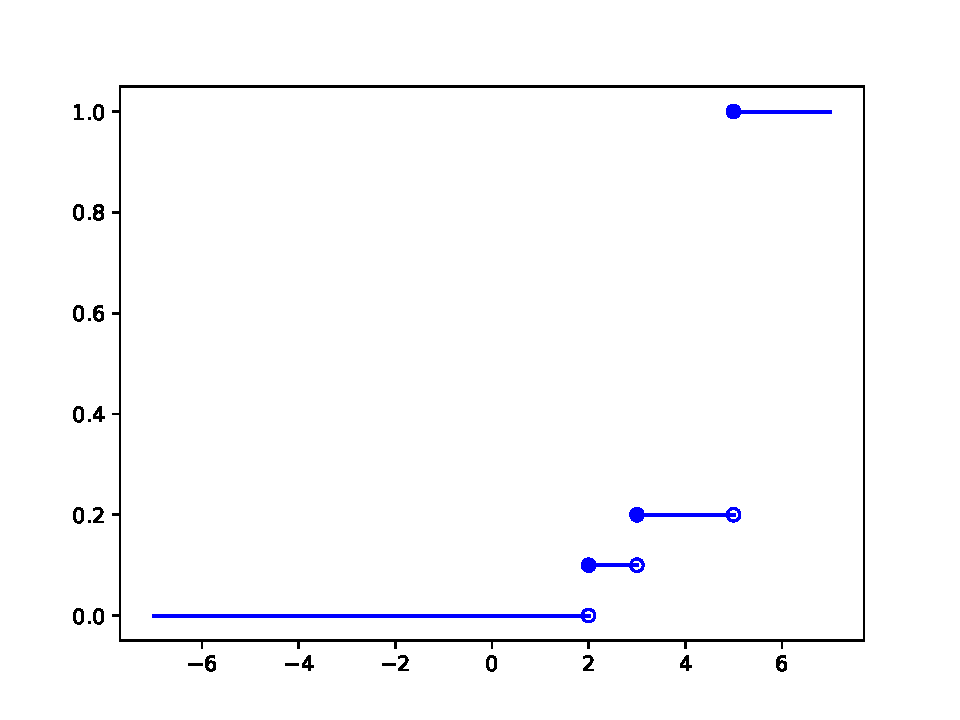
\includegraphics[width=0.5\textwidth]{2.pdf}
\end{figure}

\item[(4)]

\begin{enumerate}[(a)]
\item The CDF $F_X(x)$ is equal to $0$ at $x=0$, $1/4$ at $x=1$, $1/4$ at $x=3$,
and $1$ at $x=5$. It interpolates between these values affinely. I.e.

\[
F_X(x) =
\begin{cases}
0 & x \leq 0 \\
1/4x & 0\leq x\leq 1\\
1/4 & 1\leq x \leq 3 \\
1/4 + 3/8(x-3) & 3\leq x \leq 5\\
1 & x\geq 5
\end{cases}
\]

\item We will compute $F_Y(y)$ and take its derivative to compute $f_Y(y)$.
We want to calculate $F_Y(y)=\P(Y\leq y)=\P(1/X \leq y)$. This is 0 if $y\leq 0$
so we may assume without loss of generality that $y>0$.
We consider the set $A_y=\{x>0:1/x\leq y\}$. This is equal to $[1/y,\infty)$,
so $F_Y(y)=\int_{1/y}^\infty f_X(x)dx$.

First consider the case $1/y \geq 5$ i.e. $y\leq 1/5$. Then we have
\[
F_Y(y) = \int_{1/y}^\infty f_X(x)dx \leq \int_5^\infty f_X(x)dx=0.
\]
Now consider the case $3\leq 1/y\leq 5$ i.e. $1/5\leq y\leq 1/3$.
Since $1/y \geq 3$ we have
\[
F_Y(y) =  \int_{1/y}^5 \frac{3}{8} dx
=\frac{3}{8}(5-1/y).
\]
Now consider the case $1\leq 1/y\leq 3$ i.e. $1/3\leq y\leq 1$.
Since $1/y \geq 1$ we have
\[
F_Y(y) = \int_{1/y}^\infty f_X(x)dx = \int_3^5 \frac{3}{8} dx=\frac{3}{4}.
\]
Finally if $0<1/y\leq 1$, i.e. $1\leq y$, we have
\[
F_Y(y) = \int_{1/y}^1 f_X(x) dx + \frac{3}{4}
= \frac{1}{4}(1-1/y) + \frac{3}{4}.
\]
\end{enumerate}

Thus,
\[
F_Y(y) =
\begin{cases}
0 & y\leq 1/5 \\
\frac{3}{8}(5-\frac{1}{y}) &  1/5 \leq y\leq 1/3 \\
\frac{3}{4} & 1/3 \leq y \leq 1 \\
\frac{3}{4} + \frac{1}{4}(1-\frac{1}{y}) & y\geq 1
\end{cases}
\]
and
\[
f_Y(g) =
\begin{cases}
0 & y\leq 1/5 \\
\frac{3}{8y^2} &  1/5 \leq y\leq 1/3 \\
0 & 1/3 \leq y \leq 1 \\
\frac{1}{4y^2} & y\geq 1.
\end{cases}
\]

\item[(7)]

We have $\P(Z>z) = \P(X>z \text{ and } Y>z)=\P(X>z)\P(Y>z)$ by independence.
This is equal to $(1-F_X(z))(1-F_Y(z))$ and
\[
F_X(z)=F_Y(z) =
\begin{cases}
0 & z\leq 0 \\
z & 0\leq z \leq 1\\
1 & z\geq 1.
\end{cases}
\]
Thus \[
F_Z(z) = 1-(1-F_X(z))(1-F_Y(z)) =
\begin{cases}
0 & z\leq 0 \\
2z-z^2 & 0\leq z \leq 1\\
1 & z\geq 1
\end{cases}
\]
and
\[
f_Z(z) =
\begin{cases}
2 - 2z & 0\leq z \leq 1\\
0 & \text{otherwise}.
\end{cases}
\]

\item[(8)]

If $x\geq 0$ then $X^+ > x$ if and only if $X>x$. Thus $F_{X^+}(x)=F(x)$.

If $x<0$ then $X^+>x$ automatically. So $F_X^+(x)=\P(X^+\leq x)=0$.

Thus \[
F_{X^+}(x) =
\begin{cases}
0 & x < 0 \\
F_X(x) & x\geq 0.
\end{cases}
\]

\item[(9)]

We have $f_X(x)=\frac{1}{\beta} e^{-x/\beta}$ for $x > 0$.
Thus if $x>0$
\[
F_X(x) = \int_{\infty}^x f_X(t)dt = 1-e^{-x/\beta}.
\]
In general,
\[
F_X(x) =
\begin{cases}
0 & x \leq 0 \\
1-e^{-x/\beta} & x\geq 0.
\end{cases}
\]

For $0\leq q\leq 1$, $F_X^{-1}(q) = \inf \{x : F_X(x) \geq q\}$. Solving
$1-e^{-x/\beta} \geq q$ for $x$ yields $x\geq -\beta\log(1-q)$. So
$F_X^{-1}(q)=-\beta\log(1-q)$.

\item[(11)]

\begin{enumerate}[(a)]
\item $\P(X=1, Y=1)=0$ but $\P(X=1)=1/2$ and $\P(Y=1)=1/2$.
\item Choose $n\geq 0$. Then
\[
\P(X=n)=f_X(n) = \sum_{N=n}^\infty \frac{e^{-\lambda}\lambda^N}{N!}\binom{N}{n}.
\]
I.e. the total number of flips $N$ ranges from $n$ to $\infty$, there is
probability $e^{-\lambda}\lambda^N/N!$ for the number $N$ of flips, and
the number of possible ways for $n$ of those flips to be heads is
$\binom{N}{n}$. The above infinite sum is also equal to $f_Y(n)$.
Simplifying $\binom{N}{n}/N!$ to $\frac{1}{n!(N-n)!}$ and pulling out factors
of $e^\lambda$ and $1/n!$ from the sum yields that $f_X(n)$ is
\[
\frac{e^{-\lambda}}{n!} \sum_{N=n}^\infty \frac{(\lambda/2)^N}{(N-n)!}
= \frac{e^{-\lambda}}{n!}(\lambda/2)^n \sum_{m=0}^\infty \frac{(\lambda/2)^m}{m!}
= \frac{e^{-\lambda}}{n!}(\lambda/2)^ne^{\lambda/2}
=\frac{e^{-\lambda/2}}{n!}(\lambda/2)^n
\]

On the other hand,
\[
\P(X=m,Y=n) = f_{X,Y}(m,n) =
\frac{e^{-\lambda}\lambda^{m+n}}{(m+n)!}\binom{m+n}{m}(1/2)^{m+n}
=\frac{e^{-\lambda} (\lambda/2)^{m+n}}{m!n!}.
\]
I.e. the first term in the product is the probability of $m+n$ total flips
and the second term is the probability of seeing $m$ heads and $n$ tails among
these flips. By our simplified expression for $f_X$ and $f_Y$ we see that
the above expression for $\P(X=m,Y=n)$ is equal to $\P(X=m)\P(Y=n)$
and $X$ and $Y$ are indeed independent.
\end{enumerate}

\item[(13)]

\begin{enumerate}[(a)]
\item The PDF for $X$ is
\[
f_X(x)=\frac{1}{\sqrt{2\pi}}e^{-x/2}.
\]
We have
\[
F_Y(y)=\P(Y\leq y)=\P(e^X\leq y)=F_X(\log(y))=
\int_{-\infty}^{\log(y)} \frac{1}{\sqrt{2\pi}}e^{-x^2/2}dx
\]
for $y>0$ and $F_Y(y)=0$ elsewhere.
The derivative is
\[
f_Y(y) = \frac{1}{y}\frac{1}{\sqrt{2\pi}}e^{-\log^2y/2}
\]
for $y>0$ and $F_Y(y)=0$ elsewhere.

\item

See the Jupyter Notebook:
\href{https://github.com/ajrasmus/some_of_statistics/blob/main/chapter_2/13.ipynb}{13.ipynb}
\end{enumerate}

\item[(14)]
We have
\[
F_R(r) = \P(\sqrt{x^2+y^2}\leq r)=
\begin{cases}
0 & r \leq 0 \\
r^2 & 0 \leq r \leq 1 \\
1 & r \geq 1
\end{cases}
\]
i.e. this is the area of the disk of radius $r$ after normalizing so that the
unit disk has area 1 by dividing by its usual area, $\pi$.
Taking the derivative yields
\[
f_R(r) = \begin{cases}
2r & 0\leq r \leq 1 \\
0 & \text{otherwise}.
\end{cases}
\]

\item[(15)]

Since $F$ is continuous and strictly increasing, $F^{-1}$ exists as a function
$F^{-1}:(0,1)\to \R$. For $0\leq y \leq 1$ we have
\[
F_Y(y) = \P(F(X) \leq y) = \P(X \leq F^{-1}(y)) = F(F^{-1}(y))=y.
\]
So
\[
F_Y(y) =
\begin{cases}
0 & y \leq 0 \\
y & 0\leq y\leq 1 \\
1 & y\geq 1 \\
\end{cases}
\]
and $f_Y = \chi_{[0,1]}$, the indicator function of $[0,1]$.

If $U\sim \Unif(0,1)$ and $X=F^{-1}(U)$ then
\[
F_X(x) = \P(F^{-1}(U) \leq x) = \P(U \leq F(x)) =
\begin{cases}
0 & F(x) \leq 0 \\
F(x) & 0\leq F(x) \leq 1 \\
1 & F(x) \geq 1
\end{cases}
\]
Of course the first and third cases are vacuous, so $F_X(x)=F(x)$.

Now we consider the case $F(x)=-e^{-x/\beta}+1$, the CDF for the exponential
distribution. The inverse of this function is $F^{-1}:(0,1)\to \R$,
$F^{-1}(y) = -\beta \log(1-y)$. So if $U\sim \Unif(0,1)$ then
$F^{-1}(U)\sim \Exp(\beta)$.

See the Jupyter Notebook
\href{https://github.com/ajrasmus/some_of_statistics/blob/main/chapter_2/13.ipynb}{15.ipynb}
for a demo.

\item[(16)]
We consider conditional probability distributions:
\[
f_{X|X+Y}(x|n) = \frac{f_{X,X+Y}(x,n)}{f_{X+Y}(n)}.
\]
We have $f_{X,X+Y}(x,y) = \P(X=x, X+Y=n) = \P(X=x) \P(Y = n-x)=f_X(x)f_Y(n-x)$.
Plugging in for $f_X$, $f_Y$, and $f_{X+Y}$ and noting that
$X+Y\sim \Poiss(\lambda+\mu)$ yields that $f_{X|X+Y}(x|n)$ is equal to
\[
\frac{e^{-\lambda}\frac{\lambda^x}{x!}e^{-\mu}\frac{\mu^{n-x}}{(n-x)!}}
{e^{-\lambda-\mu}\frac{(\lambda+\mu)^n}{n!}}
=
\binom{n}{x} \left(\frac{\lambda}{\lambda+\mu}\right)^x\left(\frac{\mu}{\lambda+\mu}\right)^{n-x}
= \binom{n}{x} (\lambda/\pi)^x (1-\lambda/\pi)^{n-x}.
\]
This is exactly the expression for the PDF of $\Binom(n,\pi)$ at $x$.

\item[(17)]
We plug in $y=1/2$ and consider the resulting distribution. We have
\[
\P\left(X<\frac{1}{2} | Y = \frac{1}{2}\right)
= \int_0^{1/2} \frac{c(x+1/4)}{f_Y(1/2)}dx
= \frac{c}{4f_Y(1/2)}
\]

So we need to compute the marginal distribution $f_Y(y)$. We have
\[
f_Y(y) = \int_0^1 c(x+y^2)dx = c\left(\frac{1}{2}+y^2\right)
\]
To compute $c$ we solve
\[
1 = \int_0^1 \int_0^1 c(x+y^2)dxdy = \int_0^1 \left(\frac{1}{2}c + cy^2\right)dy
= \frac{1}{2}c + \frac{1}{3}c = \frac{5}{6}c.
\]
Thus $c = \frac{6}{5}$. Finally we can plug in to find
\[
f_Y\left(\frac{1}{2}\right) = \frac{6}{5}\left(\frac{1}{2}+\frac{1}{4}\right)
= \frac{9}{10} \text{ and }
\P\left(X<\frac{1}{2} | Y = \frac{1}{2}\right) = \frac{6/5}{4 \cdot 9/10} =
\frac{1}{3}.
\]

\item[(18)]
See the Jupyter Notebook:
\href{https://github.com/ajrasmus/some_of_statistics/blob/main/chapter_2/18.ipynb}{18.ipynb}
\end{enumerate}
\end{document}
